\documentclass[10pt,a4paper]{article}
\usepackage[T2A]{fontenc}
\usepackage[utf8]{inputenc}
\usepackage[english,russian]{babel}
\usepackage[margin=2cm]{geometry}
\usepackage{amsmath,amssymb}
\usepackage{graphicx,booktabs,array,xcolor}
\usepackage[hidelinks]{hyperref}
\usepackage{caption}
\captionsetup{font=small,labelfont=bf}
\setlength{\parskip}{3pt}
\newcommand{\mg}{\mathrm{MG}}
\newcommand{\good}[1]{\textcolor[HTML]{117733}{#1}}
\newcommand{\bad}[1]{\textcolor[HTML]{BB5566}{#1}}
\graphicspath{{../}{../../}}

\title{MG по скалярному логу как дешёвый детектор упрощения обучения:\\
что работает. Итоговый отчёт}
\author{Проект 202, эксперименты 29 сентября --- 1 октября 2026}
\date{}

\begin{document}
\maketitle

\section*{Коротко}

Метод по теории считает число активных компонент детерминированного возвратного
режима, и на синтетических системах так и происходит. На реальном обучении его
прикладная роль скромнее и практичнее: \textbf{дешёвый детектор упрощения}, который
работает по одному уже записанному логу. Ниже собрано, что эту роль подтвердили
эксперименты этой серии: MLP на digits, свёрточная сеть на CIFAR-10 и ResNet-18 на
полном CIFAR-10. Упрощение в каждом случае установлено независимо --- построением
события или дорогим измерением по всем весам.

\begin{enumerate}\setlength\itemsep{2pt}
\item \textbf{Явные события упрощения в обучении CNN.} Заморозка сети, прунинг,
  сильный спад learning rate дают \good{$-12\ldots-19\,\%$} MG; контроли без упрощения
  --- $0\ldots+13\,\%$. Разделение: AUC 0.93, для сильнейших доз 0.99. Простые
  статистики того же лога дают AUC $\approx 0.5$. Результат повторён на сидах,
  которые не участвовали в выборе настроек.
\item \textbf{Онлайн-детектор.} Порог выбран на одних сидах и проверен на других:
  \good{27 из 28} запусков с сильным упрощением пойманы, \good{0 из 16} ложных тревог,
  задержка около 1\,000 шагов. Детекторы на простых статистиках ложно срабатывают в
  31--62\,\% запусков без упрощения.
\item \textbf{Специфичность.} MG не реагирует на масштаб лога и не принимает за
  упрощение ни сглаживание лога, ни уменьшение шума градиента. На ResNet-18 ---
  \good{0 ложных тревог в 24} запусках без упрощения при \good{6 из 6} пойманных
  заморозках ($-28\ldots-31\,\%$).
\item \textbf{Информация сверх спектра.} На логе нормы параметров MG заметно ниже,
  чем у суррогата с тем же спектром (отношение 0.78--0.80), и его сдвиг при событиях
  суррогат не повторяет. В полнобатчевом обучении с большим шагом отношение
  0.51--0.66, и MG устойчив к сглаживанию лога, а спектральные статистики --- нет.
\item \textbf{Цена.} 5--10 мс на окно лога; лог нормы параметров не требует ни
  одного прохода сети и занимает десятки килобайт. Дорогие эталоны требуют хранить
  все веса (450--560 МБ на запуск) или десятки произведений Гессиана на вектор на
  каждый чекпойнт.
\end{enumerate}

\section{Что значит «работает» и как это проверялось}

\paragraph{Что меряется.} Оценка MacKay--Ghahramani по delay-реконструкции одного
скаляра (реализация проекта без изменений ядра), в скользящих окнах. Сравнивается
её значение до события упрощения и после, либо её ход во времени с независимо
измеренным упрощением.

\paragraph{Независимое подтверждение упрощения.}
\begin{itemize}\setlength\itemsep{0pt}
\item \emph{по построению} --- число обучаемых или ненулевых параметров, шаг
  оптимизатора;
\item \emph{дорогим измерением} --- PR ковариации обновлений всех весов (на
  ResNet-18 через CountSketch); доля движущихся параметров; средний размер
  обновления.
\end{itemize}

\paragraph{Контроли, где упрощения нет.} Масштаб лога (MG обязан не измениться);
сглаживание лога при той же траектории; увеличенный батч --- меньше шума градиента
при тех же движущихся параметрах. Детектор, который путает эти случаи с упрощением,
бесполезен на практике.

\paragraph{Защита от подгонки.} Протоколы с предсказаниями записывались до
запусков (docstring скриптов, \texttt{PROTOCOL.md}). Выбор наблюдателя и настроек
делался на одних сидах, проверка --- на других. Сравнение идёт с простыми
статистиками того же лога (пересечения тренда, автокорреляция, разброс),
откалиброванными тем же способом.

\section{Где у MG есть своя информация (MLP, digits)}

Первые два эксперимента проверяли, что именно MG видит в логе обучения. Сеть ---
MLP $64\!-\!64\!-\!64\!-\!10$ на sklearn digits. Для каждого окна считалось отношение
MG к MG IAAFT-суррогата --- ряда с тем же спектром, но без нелинейной структуры.

\begin{figure}[h]
\centering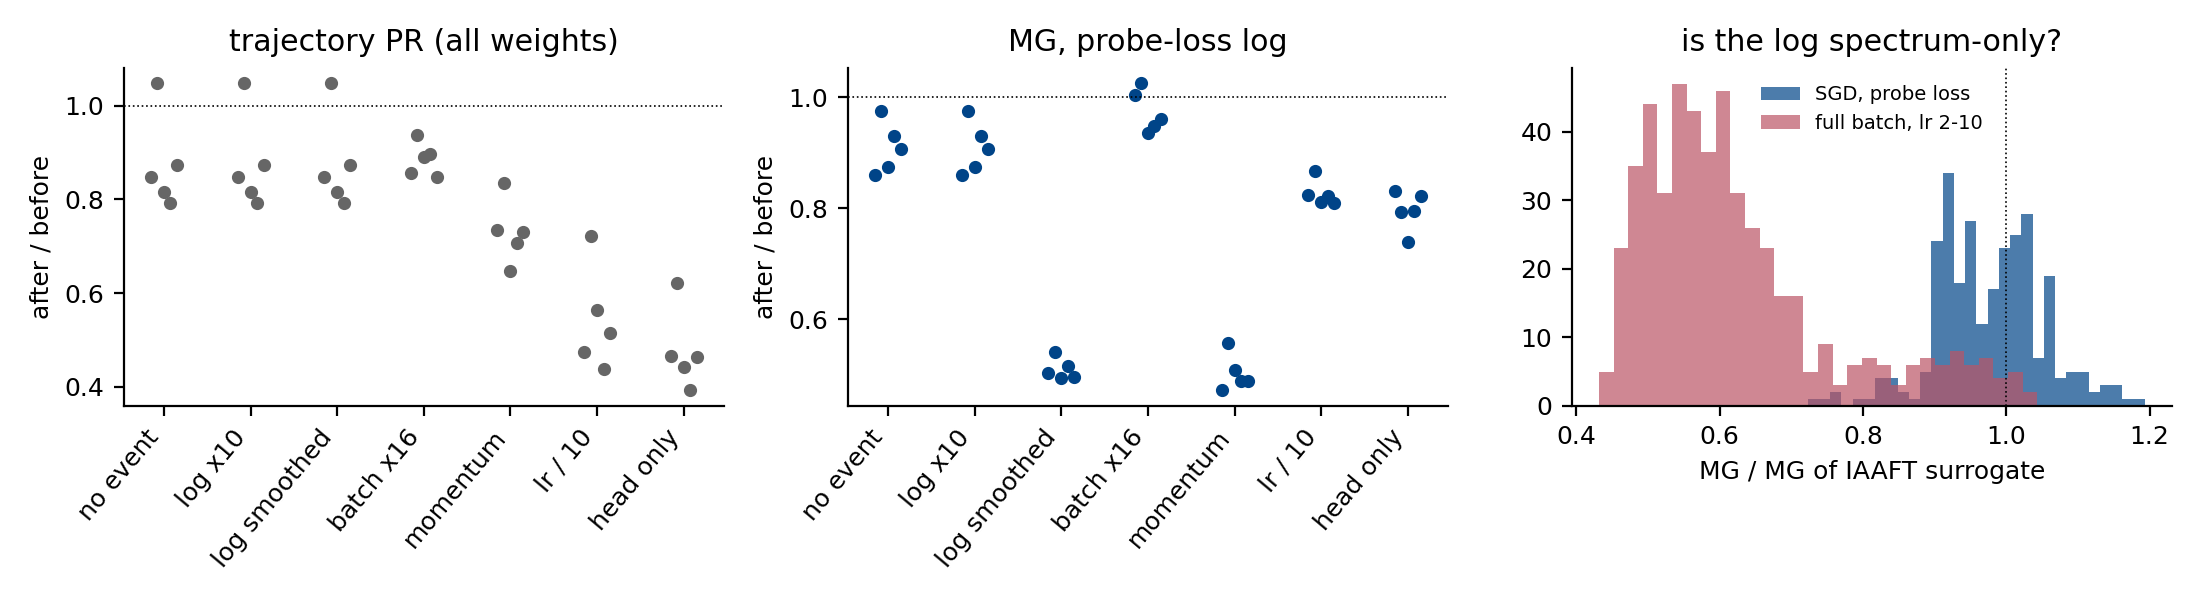
\includegraphics[width=\textwidth]{report/pilot_summary.png}
\caption{Слева и в центре --- отношение после/до для PR траектории всех весов и для
MG лога loss при событиях под SGD. Справа --- отношение MG к MG суррогата: под
SGD около 1, в полнобатчевом режиме с большим шагом --- заметно ниже 1.}
\end{figure}

\begin{itemize}\setlength\itemsep{1pt}
\item \textbf{Под SGD MG ранжирует события правильно.} Спад lr и заморозка, при
  которых PR траектории падает вдвое, снижают MG лога loss (AUC 0.99, корреляция
  отношений с эталоном $\rho=0.85$). Масштаб лога и меньший шум MG не снижают.
\item \textbf{В детерминированном режиме у MG есть информация сверх спектра.} При
  полнобатчевом обучении с большим шагом loss колеблется сам, без шума выборки, и MG в
  1.5--2 раза ниже суррогатного. Сглаживание лога меняет MG слабо (0.87--1.15), а
  MG суррогата и пересечения тренда падают (0.62--0.80 и 0.27--0.56). Здесь MG видит
  то, чего не видят спектральные статистики.
\end{itemize}

Эти наблюдения определили следующие шаги: эталоном должно быть движение весов, а
наблюдателем --- лог, в котором сохраняется нелинейная структура. Таким
наблюдателем оказалась норма параметров.

\section{Явные события упрощения в обучении CNN (CIFAR-10)}

\paragraph{Постановка.} Свёрточная сеть (14\,666 параметров), CIFAR-10 (10\,000
изображений), SGD с momentum. На шаге 4\,000 из 10\,000 --- одно событие.
Наблюдатель --- норма всех параметров: считается по уже имеющимся весам за $O(P)$,
без прохода сети. Настройки (конфигурация статьи $E=20$, $k=20$, окно 1\,000 шагов)
выбраны на сидах 0--3 и затем проверены на новых сидах 10--13.

\begin{table}[h]\centering\footnotesize
\begin{tabular}{lcccc}\toprule
событие & MG до $\to$ после & изменение (разброс по сидам) & PR обновлений & движется\\\midrule
без события & $4.31\to4.32$ & $+0.4\,\%$ ($-8.7\ldots+3.3$) & $+40\,\%$ & 100\,\%\\
батч $\times4$ (меньше шума) & $4.31\to4.85$ & $+12.8\,\%$ ($+8.3\ldots+13.9$) & $-7\,\%$ & 100\,\%\\
лог $\times10$ / лог сглажен & $4.31\to4.32$ / $4.44$ & $+0.4$ / $+3.4\,\%$ & --- & ---\\\midrule
lr $/10$ & $4.31\to3.95$ & $\mathbf{-8.3\,\%}$ ($-12.1\ldots-2.3$) & $-22\,\%$ & 100\,\%\\
lr $/100$ & $4.31\to3.85$ & $\mathbf{-11.5\,\%}$ ($-14.4\ldots-7.3$) & $-21\,\%$ & 100\,\%\\
обучается только голова & $4.31\to3.51$ & $\mathbf{-18.5\,\%}$ ($-24.1\ldots-11.2$) & $-43\,\%$ & 2.2\,\%\\
обучается только bias головы & $4.31\to3.58$ & $\mathbf{-16.7\,\%}$ ($-23.7\ldots-15.0$) & $-68\,\%$ & 0.07\,\%\\
прунинг 50\,\% & $4.31\to3.80$ & $\mathbf{-12.7\,\%}$ ($-14.5\ldots-3.9$) & $+15\,\%$ & 50\,\%\\
прунинг 80\,\% & $4.31\to3.59$ & $\mathbf{-17.5\,\%}$ ($-20.7\ldots-12.3$) & $-10\,\%$ & 20\,\%\\
прунинг 95\,\% & $4.31\to3.79$ & $\mathbf{-11.5\,\%}$ ($-16.1\ldots-9.5$) & $-45\,\%$ & 6\,\%\\
\bottomrule\end{tabular}
\caption{Медиана по 4 новым сидам. PR обновлений и доля движущихся параметров ---
дорогое независимое подтверждение: для них нужны все веса на каждом шаге.}
\end{table}

\begin{figure}[h]
\centering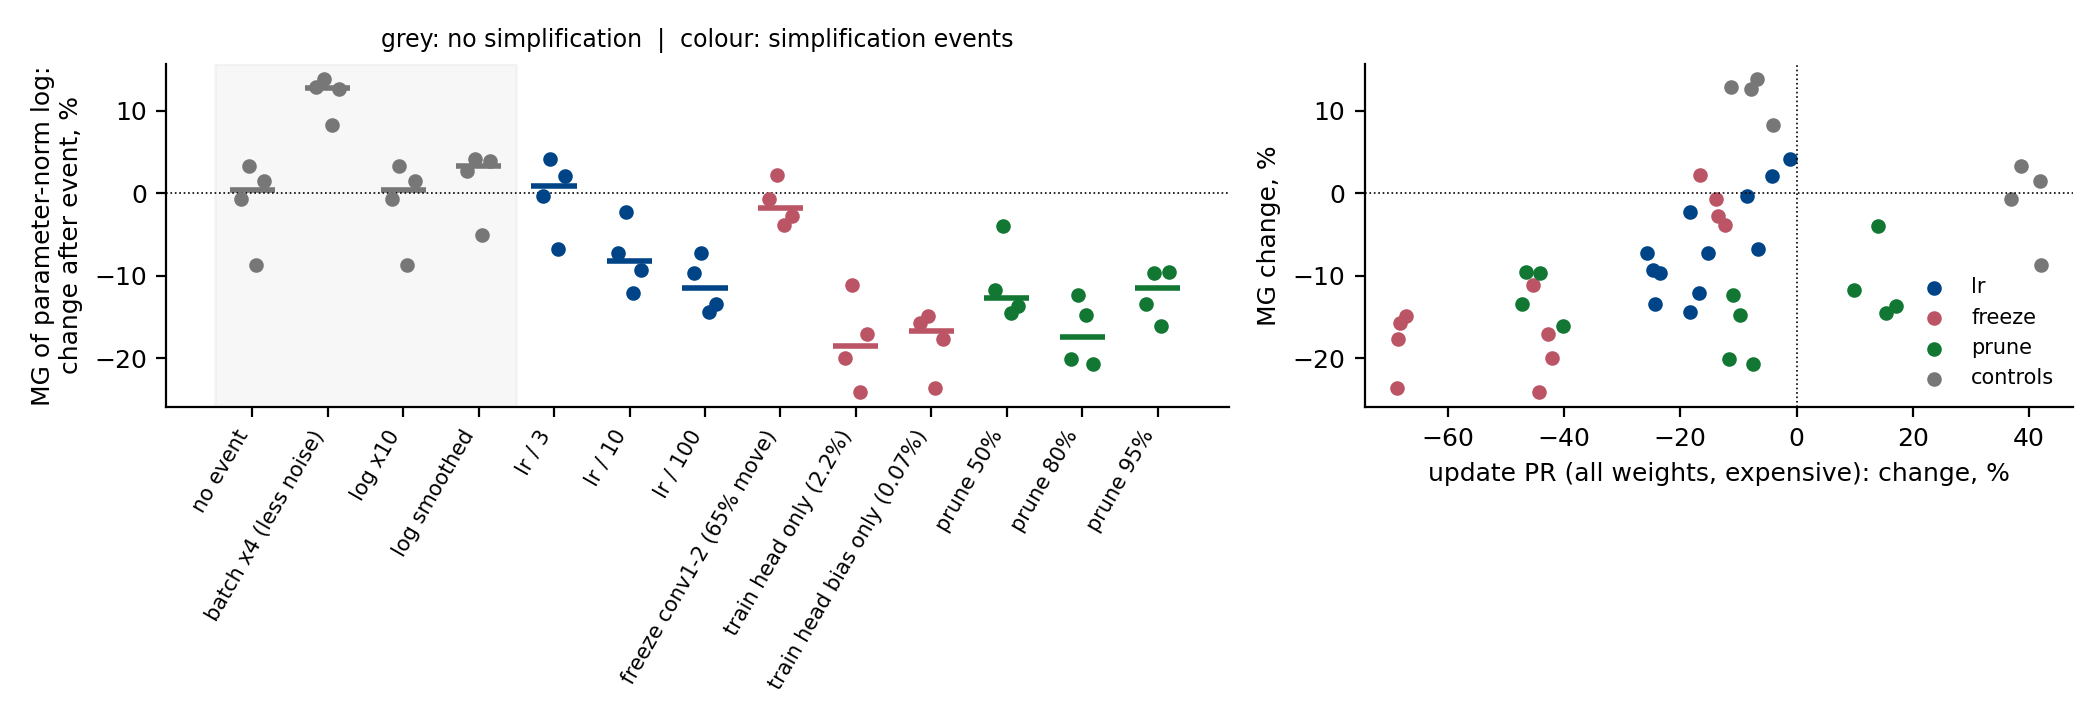
\includegraphics[width=\textwidth]{results_graded/figures/mg_change.png}
\caption{Изменение MG после события по каждому запуску. Серый фон --- контроли без
упрощения. Справа --- против изменения PR обновлений всех весов.}
\end{figure}

\paragraph{Что в этом хорошего.}
\begin{itemize}\setlength\itemsep{1pt}
\item \textbf{Все сильные события} (lr$/10$, lr$/100$, заморозка, прунинг) снижают MG;
  контроли его не снижают. При этом уменьшение шума (батч$\times4$) сдвигает MG
  \emph{вверх}, так что метод отличает «меньше направлений» от «меньше шума».
\item \textbf{Доза и ответ.} Внутри семейства спада lr ($\rho=-0.83$) и заморозки
  ($-0.68$) эффект растёт с силой упрощения. Изменение MG согласуется с изменением PR
  обновлений всех весов ($\rho=0.59$ по всем запускам).
\item \textbf{Преимущество над простыми статистиками.} AUC «событие против контроля»:
  MG 0.93, для сильнейших доз 0.99. Пересечения тренда, автокорреляция и разброс
  того же лога дают 0.48--0.67.
\item \textbf{Нелинейная информация.} MG заметно ниже, чем у суррогата с тем же
  спектром (отношение 0.78), а сдвиг MG при событиях не повторяется у суррогата
  (AUC 0.68 против 0.93). Метод видит в логе структуру, которой нет в спектре.
\end{itemize}

\section{Онлайн-детектор}

На практике момент события неизвестен, поэтому нужен монитор, который сам поднимает
тревогу. Правило: медиана MG последних 2 окон сравнивается с медианой 3 окон перед
ними, тревога --- при падении больше чем на 8.8\,\%. Порог выбран на сидах 0--3 так,
чтобы там не было ни одной ложной тревоги, и без изменений применён к сидам 10--13.

\begin{center}\small
\begin{tabular}{lcccc}\toprule
детектор на & сильные события пойманы & ложные тревоги без упрощения & задержка\\\midrule
\textbf{MG} & \good{\textbf{27/28}} & \good{\textbf{0/16}} & 1\,000 шагов\\
разброс лога & 28/28 & \bad{10/16} & 500 шагов\\
пересечения тренда & 15/28 & \bad{5/16} & 1\,000 шагов\\
автокорреляция & 0/28 & 0/16 & ---\\
\bottomrule\end{tabular}
\end{center}

Только MG одновременно ловит почти все сильные упрощения и ни разу не срабатывает
без причины. Разброс лога ловит всё, но срабатывает и на масштабировании лога, и
на обычном обучении.

\begin{figure}[h]
\centering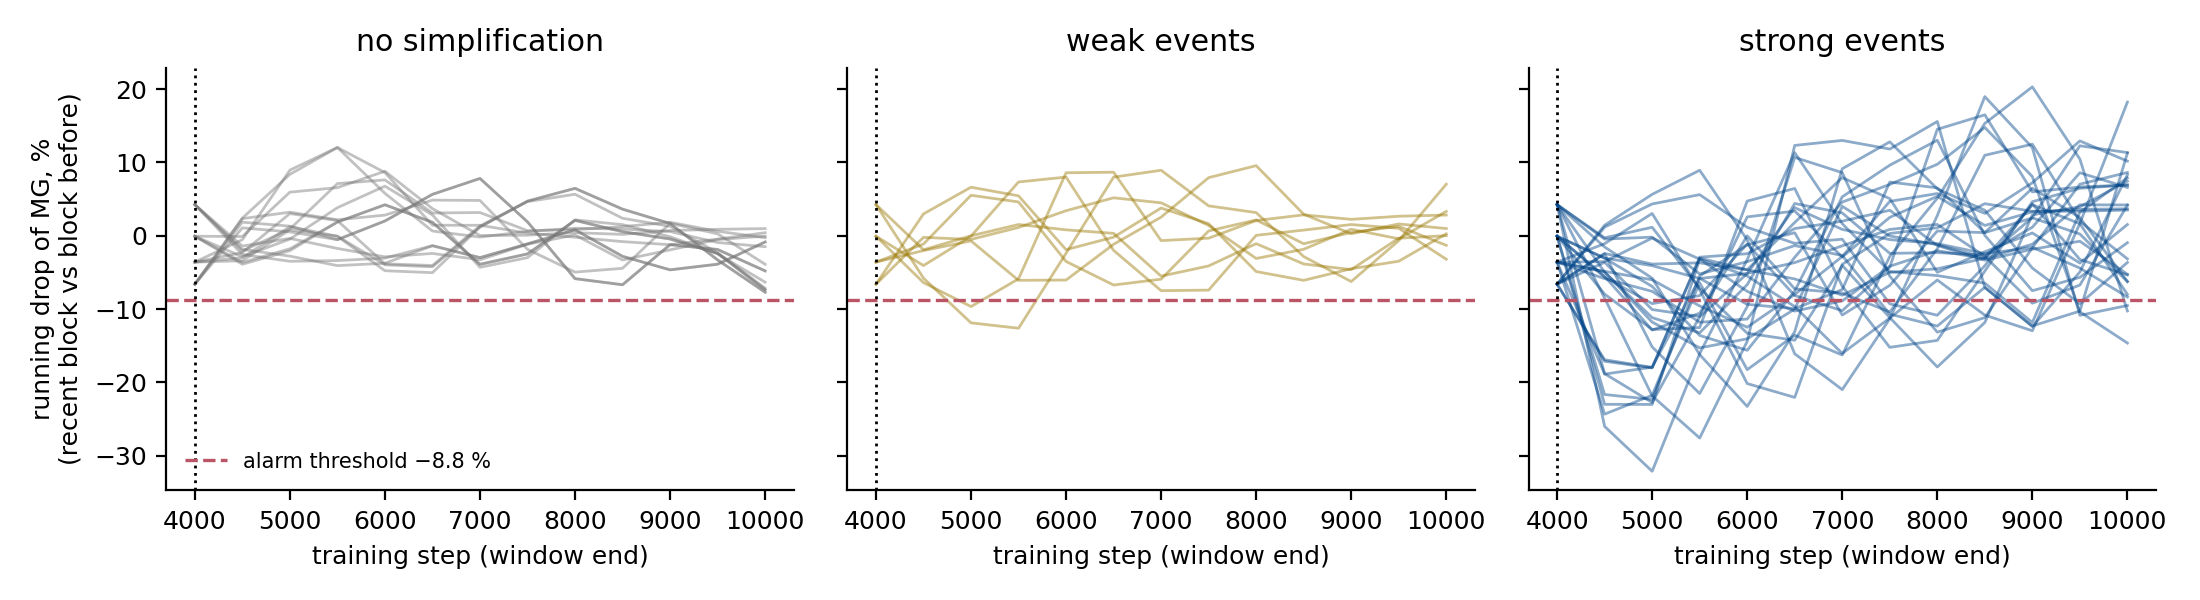
\includegraphics[width=\textwidth]{results_detector/detector_traces.png}
\caption{Статистика детектора по всем тестовым запускам. Пунктир --- порог $-8.8\,\%$,
выбранный на других сидах.}
\end{figure}

\section{ResNet-18 на полном CIFAR-10: заморозка без ложных тревог}

ResNet-18 (11 млн параметров) обучалась на полном CIFAR-10 в двух сценариях: с нуля и
дообучение ImageNet-предобученной модели --- типичный сценарий transfer learning.
Протокол записан до запуска; настройки MG и правило детектора перенесены без
изменений с малой CNN.

\begin{figure}[h]
\centering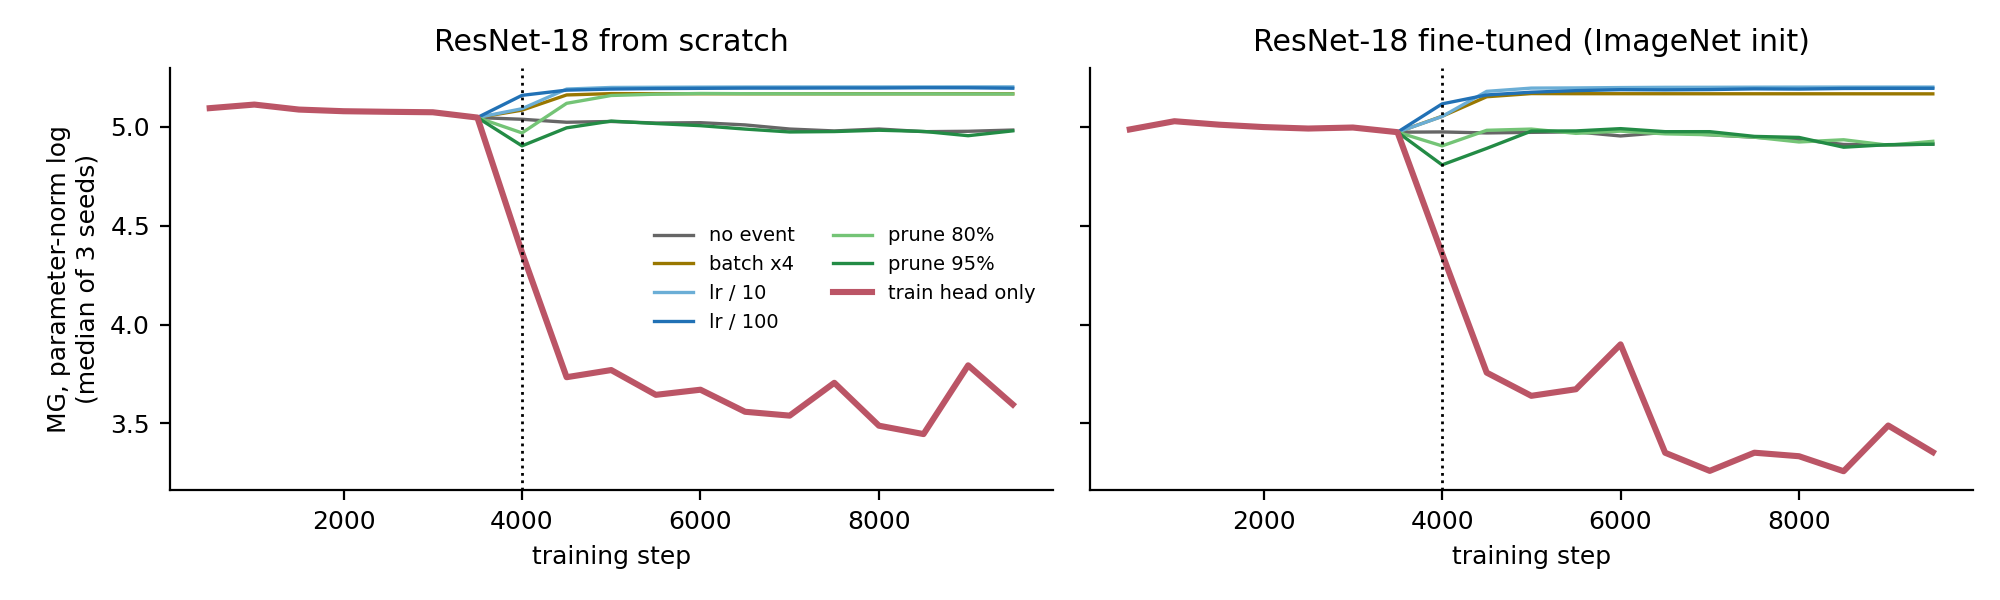
\includegraphics[width=\textwidth]{report_final/resnet_freeze.png}
\caption{MG лога нормы параметров ResNet-18. Заморозка всего, кроме головы
(красная линия), видна сразу и в обоих сценариях.}
\end{figure}

\begin{itemize}\setlength\itemsep{1pt}
\item Заморозка всего, кроме головы, снижает MG на \good{$27.6\,\%$} при обучении с
  нуля и на \good{$30.8\,\%$} при дообучении. Детектор с порогом, выбранным ещё на
  малой CNN, ловит её \good{в 6 из 6} запусков.
\item \good{Ни одной ложной тревоги} в 24 запусках без упрощения (без события,
  меньший шум, масштаб и сглаживание лога, оба сценария).
\item Правило детектора перенеслось с сети в 15 тыс. параметров на сеть в 11 млн
  без повторной калибровки.
\end{itemize}

\section{Цена}

\begin{center}\small
\begin{tabular}{p{7.2cm}p{8.6cm}}\toprule
что нужно & цена\\\midrule
\textbf{MG одного окна лога} (500--1\,000 точек) & \textbf{5--10 мс} на CPU\\
\textbf{лог нормы параметров} & $O(P)$ на шаг, без прохода сети; 31--39 КБ на запуск\\
эффективный ранг / PR траектории или обновлений & все веса на каждом шаге: 450--560 МБ на запуск малой CNN; 180--300 мс на окно\\
PR обновлений ResNet-18 через CountSketch & 1\,024 числа на шаг вместо 11 млн, но скетч надо считать на каждом шаге обучения\\
верхние собственные значения Гессиана & $\approx 100$ мс и $\approx 60$ произведений Гессиана на вектор на чекпойнт\\
\bottomrule\end{tabular}
\end{center}

\section{Как формулировать в статье}

\begin{quote}
По теории оценка считает число активных компонент детерминированного возвратного
режима, и на синтетических системах так и происходит. На реальном обучении та же
оценка по одному уже записанному скалярному логу --- норме параметров --- работает
как дешёвый детектор упрощения. При явных событиях упрощения в обучении свёрточной
сети (заморозка, прунинг, спад learning rate) она снижается на 12--19\,\%, не
реагируя на масштаб лога, его сглаживание и уменьшение шума градиента; простые
статистики того же лога эти события не отделяют. Онлайн-детектор с порогом,
выбранным на других запусках, ловит 27 из 28 таких событий без ложных тревог, а на
ResNet-18 --- заморозку сети во всех запусках, тоже без ложных тревог. Теория и
синтетика позволяют читать изменение оценки как относительное изменение числа
активных направлений, хотя абсолютное значение размерностью не является.
\end{quote}

\section{Границы применимости}

Чтобы формулировка выдерживала вопросы рецензентов, эти ограничения надо указать
явно. Все они описаны подробно в \texttt{research\_trajectory\_reference/report/}.
\begin{itemize}\setlength\itemsep{1pt}
\item \textbf{Не размерность.} Абсолютное значение MG на реальном обучении
  размерностью не является: отношение идентифицируемости $\approx 1.5$. Метод
  работает как относительный сигнал «до/после».
\item \textbf{Нужны явные упрощения.} Слабые события (lr$/3$, заморозка двух первых
  слоёв) не ловятся.
\item \textbf{Выбор лога важен.} Loss мини-батча бесполезен. MG по loss на
  фиксированной выборке сводится к спектру и ложно срабатывает при сглаживании.
  Рабочий наблюдатель --- норма параметров.
\item \textbf{Масштаб.} На ResNet-18 норма всей сети превращается в гладкую кривую,
  и MG ловит только заморозку. Спад lr и прунинг он не видит, а более шумные
  наблюдатели (случайные проекции, нормы слоёв) дают ложные тревоги. Пример с CNN
  --- это малая модель.
\item \textbf{Edge of stability.} Число колеблющихся мод Гессиана MG не считает:
  связь обратная.
\end{itemize}

\section*{Где лежат материалы}
\small
\begin{itemize}\setlength\itemsep{0pt}
\item CNN, детектор, ResNet: \texttt{research\_trajectory\_reference/}\newline
  (\texttt{cifar\_graded.py}, \texttt{detector.py}, \texttt{colab\_resnet/},
  \texttt{e7b\_analyse.py}); полный отчёт по всем экспериментам, включая
  отрицательные, --- \texttt{report/report\_all\_ru.pdf};
\end{itemize}

\end{document}
